\documentclass[12pt]{article}
\usepackage{amsmath,amsfonts,nicefrac}
\usepackage{graphicx}
\usepackage{enumerate}
\usepackage{natbib}
\usepackage{url} % not crucial - just used below for the URL 
\usepackage{ifthen}

%\pdfminorversion=4
% NOTE: To produce blinded version, replace "0" with "1" below.
\newcommand{\blind}{1}
% DON'T change margins - should be 1 inch all around.
\addtolength{\oddsidemargin}{-.5in}%
\addtolength{\evensidemargin}{-.5in}%
\addtolength{\textwidth}{1in}%
\addtolength{\textheight}{-.3in}%
\addtolength{\topmargin}{-.8in}%


\usepackage[table]{xcolor}% http://ctan.org/pkg/xcolor

\newcommand{\cl}[2]{\cellcolor{#1!#2}}
\newcommand{\inc}[2]{ \ifthenelse{\equal{#1}{1}}{\input{./sections/#2}}{ } }



\begin{document}

%\bibliographystyle{natbib}

\def\spacingset#1{\renewcommand{\baselinestretch}%
{#1}\small\normalsize} \spacingset{1}


%%%%%%%%%%%%%%%%%%%%%%%%%%%%%%%%%%%%%%%%%%%%%%%%%%%%%%%%%%%%%%%%%%%%%%%%%%%%%%

\if1\blind
{
  \title{\bf Towards Structured Use of Bayesian Sequential Monitoring in Clinical Trials}
  \author{Evan Kwiatkowski\textsuperscript{$\dagger$}, 
	        Eugenio Andraca-Carrera\textsuperscript{$\ddagger$},\\
					Mat Soukup\textsuperscript{$\ddagger$},
					\medskip Matthew A. Psioda\textsuperscript{$\dagger$}\thanks{The authors gratefully acknowledge \textit{please remember to list all relevant funding sources in the unblinded version}}\\
	  %
	  $\dagger$ Department of Biostatistics,
		University of North Carolina, \\
		McGavran-Greenberg Hall, CB\#7420, \\
		%
		\medskip Chapel Hill, North Carolina, U.S.A.\\
    $\ddagger$ Division of Biometrics VII, Office of Biostatistics \\
		           Center for Drug Evaluation and Research, \\
							 US Food and Drug Administration, \\
							 Silver Spring, Maryland, USA \\									
		}
  \maketitle
} \fi

\if0\blind
{
  \bigskip
  \bigskip
  \bigskip
  \begin{center}
    {\LARGE\bf Title}
\end{center}
  \medskip
} \fi

\bigskip
\begin{abstract}
The text of your abstract. 200 or fewer words.
\end{abstract}

\noindent%
{\it Keywords:}  3 to 6 keywords, that do not appear in the title
\vfill

\newpage
\spacingset{1.5} % DON'T change the spacing!



\section{Introduction}

Things to discuss:
\begin{itemize}
 \item 21\textsuperscript{st} Century Cures Act (MATT)
 \item PDUFA VI reauthorization (MATT)
 \item Expansive work already done on sequential monitoring  (EVAN -- draft on 6/21)
%\item Berry A Case for Bayesianism, Cornfield The Bayesian outlook, classical arguments for Bayes in clinical trials, not sequential monitoring in particular
%\item (1) Berry Montoring Accumulating Data, (2) Cornfield/Greenhouse On certain aspects, (3) Cornfield Sequential Trials, (4) A Bayesian Test of Some Classical Hypotheses, with Applications to Sequential Clinical Trials Jerome Cornfield 
%\item Bayes \& monitoring, based on posterior distributions
%\item First papers in Bayes sequential monitoring. Bayesian inferences not affected by frequent or continual monitoring by the likelihood principle.
%\item Papers which compare to frequentist stopping rules \& increased interpretation on role of priors.
%\item \cite{Spiegelhalter1994}
%\item \cite{Spiegelhalter1993} predictive distributions as basis for monitoring
%\item \cite{Freedman1992} choice of prior explained by showing its impact on percentiles of posterior distribution
%\item \cite{Freedman1989} The need to overcome this `\textbf{handicap}' prevents unduly early termination.
%\item \cite{Fayers1997} Choosing these two priors (skeptical, enthuastic) provides a useful \textbf{brake} against the premature termination of trials.
%\item Bayesian Adaptive Methods for Clinical Trials Berry, Carlin, Etc.
 \item Our majors contribution (EVAN -- as early as possible in introduction without having the flow appear weird -- draft on 6/21)
 \item Outline for the remaining section of the paper (EVAN -- draft on 6/21)
\end{itemize}
The theoretical foundations for the Bayesian clinical trials has been long established \cite{Cornfield1966}~\cite{Cornfield1966a}~\cite{Neyman1967}. These methods were not widely used in practice until a comprehensive framework for interpretation of results was developed through specifying prior distributions that were naturally and intuitively related to the research objectives (e.g. skeptical and enthuastic priors) \cite{Freedman1989}~\cite{Freedman1992}~\cite{Spiegelhalter1993}~\cite{Spiegelhalter1994}~\cite{Fayers1997}. (\textit{Rewrite paragraph.})

There is still potential for further utilization of Bayesian methods in the clinical trial setting. While the framework for interpretation of Bayesian clincial trials is well devloped, the details of specifying prior distributions in a natural and intuitive way is lacking. This paper presents a structured or default way to determine prior distributions based on the trial design. Our major contribution is to present methods for the default or automatic selection of prior distributions in a way that is applicable to a wide array of clinical trial designs.

\begin{enumerate}
\item Bayesian methodology is widely developed.
\item It has been applied (cite).
\item The current perspective is that Bayesian methodology is only valid when Frequentist methods are insufficient, including where enrollment is challenging (rare diseases, pediatric studies)
\item Our contribution is to show that Bayesian methods are applicable to all clinical trials. This is shown by highlighting their improved interpretation and showing their use in varied and complicated situations.
\end{enumerate}

\section{Methods}

As you introduce ideas that come from or extend other ideas in the literature, cite the relevant literature.

\subsection{Monitoring versus Estimation Priors (EVAN -- draft on 6/21)}

%\begin{itemize}
% \item Define generally in terms of $\boldsymbol\theta = \left( \gamma, \boldsymbol\psi  \right)$ where $\gamma$ is a parameter of interest
%       and $\boldsymbol\psi$ is a nuisance parameter (possible vector valued).
% \item Define \textit{Monitoring} Priors and \textit{Inference} Priors.
% \item Make connection between Inference priors and two-part mixture prior and BMA.
% \item Define \textit{Skeptical} and \textit{Enthusiastic} monitoring priors and how each would be used.
% \item I would have a generic graphic to illustrate the types of priors and the mixture.
% %\item Motivate in the context of a simple example (i.e., single parameter binary example).
%\end{itemize}

\subsubsection{Bayesian hypothesis testing based on posterior probabilities}

The Bayesian paradigm allows direct inference on a parameter of interest through specification of a model for the data generating mechanism and prior distributions for unknown quantities. Let $\mathbf{D}$ be a random variable representing the data collected in the trial with density $p(\mathbf{D}|\theta,\psi)$ where $\theta$ and $\psi$ are the unknown quantities. Let $\theta$ be the parameter of interest and $\psi$ be the unknown quantities that are not of primary importance (i.e. ``nuisance parameters"). Define the sample spaces for the unknown quantities as $\theta\in\Theta$ and $\psi\in\Psi$. 

Suppose the hypotheses under consideration are $H_0:\theta\in\Theta_0$ versus $H_1:\theta\in\Theta_1$, where $\Theta=\Theta_0\cup \Theta_1$ and $\Theta_0\cap \Theta_1=\emptyset$. These hypotheses are adjudicated based on posterior probabilities of $\theta$ by evaluating its marginal likelihood $P(\theta\in\Theta_i|\mathbf{D})=\int_{\Theta_i}p(\theta|\mathbf{D})d\theta$ for $i\in\{0,1\}$, which is marginalized over the nuisance parameters $p(\theta|\mathbf{D})=\int_{\Psi}p(\theta,\psi|\mathbf{D})d\psi$. 

Define $\delta\in[0,1]$ as a threshold for \textit{a compelling level of evidence} as it relates to $\theta$. We say that an individual is ``all but convinced" that $H_i$ is true given the observed data if $P(\theta\in\Theta_i|\mathbf{D})\geq\delta$ for $i\in\{0,1\}$. The quantity $1-\delta$ reflects \textit{residual uncertainty} of $H_i$ being true relative to the competing hypothesis. For example, an individual would be ``all but convinced" of the truth of the alternative hypothesis if $P(\theta\in\Theta_1|\mathbf{D})\geq\delta$.

The posterior distribution of $\theta$ depends on the choice of prior distribution $\pi(\theta,\psi)$ since $p(\theta,\psi|\mathbf{D})=p(\mathbf{D}|\theta,\psi)\pi(\theta,\psi)/p(\mathbf{D})$ by Bayes rule. The specification of the prior distribution depends on the research objective. An \textit{inference prior} is a prior that is used when the research objective is to make final analysis after data collection is complete. A \textit{monitoring prior} is a prior that is used when the research objective is to consider the impact of interim analyses on subject enrollment, with the potential for early termination (or less commonly prolongation).
%Possible simplifying functional relationships between $\theta$ and $\psi$ are conditional independence $\pi(\theta,\psi)=\pi(\theta|\psi)\pi(\psi)$ and independence $\pi(\theta,\psi)=\pi(\theta)\pi(\psi)$. An inference prior is often non-informative or objective in the sense that it does not show preference to $H_0$ or $H_1$. Decisions made using using a non-informative prior are often similar to those made in the frequentist setting. 

It has been said that ``the purpose of a trial is to collect data that bring to conclusive consensus at termination opinions that had been diverse and indecisive at the \textit{outset}" (Kass and Greenhouse (1989), emphasis added). These opinions manifest as priors $\pi(\theta,\psi)$ for which their relation to $P(\theta\in\Theta_i|\pi(\theta,\psi))$ $i\in\{0,1\}$ is examined. Note this quantity does not depend on the data $\mathbf{D}$ and therefore reflect a-priori opinion. A skeptical prior is an informative or subjective prior that gives substantial preference to $H_0$ such that it is ``all but convinced" that $H_0$ is true a-priori. This prior $\pi_{S}(\theta,\psi)\equiv\pi_{S}$ has the property that $P(\theta\in\Theta_0| \pi_{S})\geq\delta$ (equivalently $P(\theta\in\Theta_1| \pi_{S})<1-\delta$). The choice of $\delta\in[0,1]$ is motivated by \textit{a compelling level of evidence} as it relates to $\theta$, although in this setting the ``evidence" reflects a theoretical opinion rather than empirical judgement. For example, if $\delta=0.95$, then this choice of skeptical prior places 95\% prior probability that $\theta\in\Theta_0$. An enthuastic prior $\pi_{E}(\theta,\psi)\equiv\pi_{E}$ similarly gives preference to $H_1$ through the property that $P(\theta\in\Theta_1| \pi_{E})\geq\delta$ (equivalently $P(\theta\in\Theta_0| \pi_{E})<1-\delta$). For purposes of interpretation, a \textit{skeptical person} is someone whose a-priori opinions of $\theta$ are reflected through a skeptical prior and a \textit{enthuastic person} is someone whose a-priori opinions of $\theta$ are reflected through an ethuastic prior. The prior distributions discussed are generally ``non-informative" over the nuisance parameters.

The use of monitoring based on changing the opinion of skeptical and enthuastic priors has been described as overcoming a handicap (\cite{Freedman1989}) and providing a brake (\cite{Fayers1997}) on the premature termination of trials, or constructing ``an adversary who will need to be disilusioned by the data to stop further experimentation" (\cite{Spiegelhalter1994}). 

Early termination of the trial is appriopriate if diverse prior opinions about $\theta$ would be in agreement given the interim data (e.g. the skeptical and enthuastic person reach the same conclusion). It is then reasonable to stop data collection if, upon seeing the data, a \textit{skeptical person} changes their opinion to be ``all but convinced" that $H_1$ is true ($P(\theta\in\Theta_1|\mathbf{D}, \pi_{S})\geq\delta$), or an \textit{enthuastic person} becomes ``all but convinced" that $H_1$ is false ($P(\theta\in\Theta_0|\mathbf{D}, \pi_{E})\geq\delta$).

%Summarizing~\cite{Spiegelhalter1993} and others:  or that the benefit of treatment is not likely to be what was expected, the probability of \textit{eventually} proving that $H_1$ is true is sufficiently low, or the resources have been exhausted.  
%A standard Bayesian decision rule would reject $H_0$ when $P(\theta\in\Theta_{H_1}|D\geq 0.95)$ which will result in a Type I error rate of $0.05$ when the analysis prior is non-informative (a so-called reference or flat prior). The Bayes factor in favor of $H_0$ is defined as 
%\begin{align*}
%BF=\frac{p(D|H_0)}{p(D|H_1)}=\frac{\int_{\Theta_{H_0}}p(D|\theta,H_0)\pi(\theta|H_0)d\theta}{\int_{\Theta_{H_1}}p(D|\theta,H_0)\pi(\theta|H_1)d\theta}
%\end{align*}
%and let $p(\theta|D,\pi)$ denote the posterior distribution of $\theta$ given a particular prior distribution.


Final inference on $\theta$ is made once enrollment is stopped based on the monitoring priors or at the planned end of the trial. An inference prior $\pi_{I}(\theta,\psi)\equiv\pi_{I}$ is often non-informative or objective in the sense that it does not show a-priori preference to $H_0$ or $H_1$ ($P(\theta\in\Theta_0|\pi_I)\approx P(\theta\in\Theta_1|\pi_I)$). There are many ways to formulate an inference prior with this property. We propose use of a mixture prior constructed from the monitoring process as the inference prior:
\begin{align*}
\pi_{I}=\omega\cdot\pi_{S}+(1-\omega)\cdot\pi_E
\end{align*}
for $\omega\in[0,1]$. Choosing $\omega=1/2$ for an equal mixture of $\pi_S$ and $\pi_E$ corresponds to an inference prior that is impartial to $H_0$ and $H_1$, and is a practical choice of $\pi_I$ is to be determined before the start of data collection. Define $p(\mathbf{D}|\pi(\theta,\psi))=\int p(\theta|\mathbf{D})\pi(\theta,\psi)d(\theta,\psi)$ to be the marginal likelihood for the data given the prior $\pi(\theta,\psi)$. Choosing $\omega$ based on posterior model probabilities of the null and alternative hypotheses yields $\omega=p(\mathbf{D}| \pi_{S})/(p(\mathbf{D}| \pi_{S})+p(\mathbf{D}| \pi_{E}))$. 

All relevant information about $\theta$ can be derived from its marginal posterior distribution with an inference prior (e.g. posterior mean, credible intervals). For example, posterior mean using the inference prior will be a two-part mixture of the posterior means using the skeptical and enthuastic priors:
\begin{align*}
E(\theta|\mathbf{D},\pi_{I})=\omega\cdot E(\theta|\mathbf{D}, \pi_{S})+(1-\omega)\cdot E(\theta|\mathbf{D}, \pi_{E}).
\end{align*}


As an alternative strategy to futility analysis, one can monitor the probability of success (POS) for the trial. The probability of getting a convincing result at the end of the trail can be computed using the interim data. Let $p(\theta|\mathbf{D}, \pi_{I})$ denote the posterior distribution for $\theta$ based on the inference prior $ \pi_{I}$ and the current data $\mathbf{D}$. Let $\xi$ denote the POS which is given as follows:
\begin{align*}
\xi=E[1\{P(\theta\in\Theta_1|\mathbf{D}_1,\mathbf{D}, \pi_{I})\geq \delta\}]
\end{align*}
where the expectation is taken with respect to the posterior predictive distribution $p(\mathbf{D}_1)$ for future data $\mathbf{D}_1$ (which includes subjects yet to enroll):
\begin{align*}
p(\mathbf{D}_1)=\int p(\mathbf{D}_1|\theta)\cdot \pi(\theta|\mathbf{D})d\theta.
\end{align*}
One may stop the enrollment if $\xi$ is sufficiently small (i.e. $\xi<0.05$).
%\begin{align*}
%\pi_{Inference}=\frac{p(\mathbf{D}| \pi_{S}) \pi_{S}+p(\mathbf{D}| \pi_{E}) \pi_{E}}{p(\mathbf{D}| \pi_{S})+p(\mathbf{D}| \pi_{E})}
%\end{align*}
%\begin{align*}
%E(\theta|\mathbf{D},\pi_{Inference})=\omega\times E(\theta|\mathbf{D}, \pi_{S})+(1-\omega)\times E(\theta|\mathbf{D}, \pi_{E})
%\end{align*}
%Need to describe relation to Type I and Type II error.
%\subsubsection{Default parameterization of monitoring priors for common designs}\label{monitoring_prior_specification}
%Define prior distribution as $\pi(\theta|\lambda)$ where $\lambda$ is a vector of hyperparameters.

%Reference prior attempts to express no particular opinion about the treatment's merit. 



%\subsection{Futility Monitoring Using Probability of Success (EVAN -- draft on 6/21)}
%
%\begin{itemize}
% \item Futility monitoring using POS is about stopping early when their is a high likelihood
%       of a study being inconclusive at the end of the study.
% \item Since the final analysis uses the \textit{Inference} prior, POS should be based on the
%       inference prior.
% \item Develop the framework for POS and show how it is a weighted average POS based on the skeptical
%       and enthusiastic priors.
%\end{itemize}


%Stochastic curtailment in frequentist setting.
\section{Examples -- (EVAN)}

\subsection{Single-Arm Oncology Proof-of-Activity Trial w/ Binary Endpoint}


Consider a single-arm oncology proof-of-activity trial with a binary endpoint. The data $\mathbf{D}$ is assumed to be Binomially distributed. The response rate $\theta$ is the parameter effect of interest, which is the only unknown quantity in this simple situation.

Consider testing the hypothesis $H_0:\theta\leq\theta_0\text{ versus }H_1:\theta>\theta_0$. Using the general notation $\Theta_0=[0,\theta_0]$ and $\Theta_1=(\theta_0,1]$. Consider a highly clinically relevant treatment effect $\theta_A>\theta_0$. It is desirable that the trial have appropriate power (probability of proving $H_1$ when $\theta=\theta_A$). 

Monitoring priors for this trial will be made using the concepts of a skeptical prior and an enthuastic prior. Recall a skeptic is ``all but convinced" that $H_0$ is true a-priori, therefore $P(\theta\in\Theta_0|\pi_S)\geq\delta$. An optimist is ``all but convinced" that $H_1$ is true a-priori, therefore $P(\theta\in\Theta_1|\pi_E)\geq\delta$. 

Beta priors for $\theta$ will be used to provide closed-form expressions of the posterior distributions via Beta-Binomial conjugacy (the posterior distribution $p(\theta|\mathbf{D})$ will be Beta distributed). The Beta distribution has two shape parameters. These parameters can be determined uniquely by specifying the desired mean and variance of the distribution. It is intuitive to center the skeptical and enthuastic priors around the quantities $\theta_0$ and $\theta_A$ respectively, so that $E(\pi_S)=\theta_0$ and $E(\pi_E)=\theta_A$. The variance for the skeptical and enthuastic priors is then uniquely determined through by the choice of threshold $\delta$. In particular, let $\pi_S(\theta)\sim \mathcal{B}(\alpha,\beta)$ be Beta distributed with shape parameters $(\alpha,\beta)$. There is a single choice of $(\alpha,\beta)$ such that:
\begin{align*}
\theta_0=E(\pi_S)=\int_{\Theta}\pi_S(\theta)d\theta=\frac{\alpha}{\alpha+\beta}\text{ and }\delta=\int_{\Theta_0}\pi_S(\theta)d\theta=\int_{0}^{\theta_0}\frac{\theta^{\alpha-1}(1-\theta)^{\beta-1}}{B(\alpha,\beta)}d\theta
\end{align*}
where $B(\alpha,\beta)$ is the Beta function.

Alternatively, the variance could be determined by specifying a desired quantile of the prior distribution which would then be reflected in $\delta$. For example, suppose it is desirable that the skeptical prior places small probability $\lambda>0$ that the $\theta\geq\theta_A$, which is the highly clinically relevant treatment effect. Then there is a single choice of $(\alpha,\beta)$ such that
\begin{align*}
\theta_0=E(\pi_S)=\int_{\Theta}\pi_S(\theta)d\theta=\frac{\alpha}{\alpha+\beta}\text{ and }\lambda=\int_{\theta_A}^{1}\pi_S(\theta)d\theta=\int_{\theta_A}^{1}\frac{\theta^{\alpha-1}(1-\theta)^{\beta-1}}{B(\alpha,\beta)}d\theta,
\end{align*}
in which case $\delta=\int_{\Theta_0}\pi_S(\theta)d\theta$ is a deterministic quantity.

Motivated by a trial for Vemurafenib (\cite{Hyman2015}) let $\theta_0=0.15$ and $\theta_A=0.45$. Consider the hypotheses
\begin{align*}
H_0&:\theta\leq 0.15\\
H_1&:\theta>0.15
\end{align*}

The skeptical prior will be Beta distributed, centered around $\theta_0=0.15$, and have $2.5\%$ prior probability that $\theta>\theta_A$. Similarly, the enthuastic prior will be centered around $\theta_A=0.45$ and have $2.5\%$ prior probability that $\theta<\theta_0$. These priors are distributed as
\begin{align*}
\pi_S(\theta)&\sim\mathcal{B}(1.187,6.724)\\
\pi_E(\theta)&\sim\mathcal{B}(3.681,4.499).
\end{align*}
\begin{center}
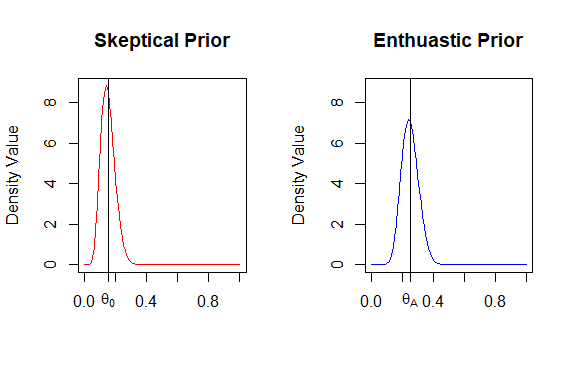
\includegraphics[width=3in]{D:/Users/ekwiatko/Documents/GitHub/Bayesian-Sequential-Monitoring/00-paper/FIGURES/figure3_1.png}
\end{center}
The trial will proceed until one of the following three conditions are satisfied:
\begin{align*}
\text{Efficacy criteria: }&P(\theta>0.15|\mathbf{D},\pi_S)\geq 0.95\\
\text{Futility criteria: }&P(\theta\leq 0.45|\mathbf{D},\pi_E)\geq 0.95\\
\text{Exhausted resources: }&N=14 \text{ patient outcomes obtained},
\end{align*}
where the maximum sample size is that of a frequentist trial design with a Type 1 error rate of $0.05$ and $80\%$ power.

The inference priors will be of the form $\pi_{I}=\omega\cdot\pi_{S}+(1-\omega)\cdot\pi_E$ with $\omega\in\{0,1/4,1/2,3/4,1\}$.
\begin{center}
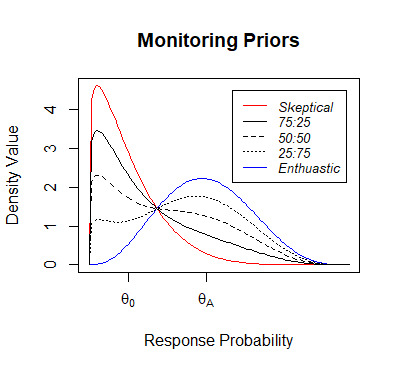
\includegraphics[width=3in]{D:/Users/ekwiatko/Documents/GitHub/Bayesian-Sequential-Monitoring/00-paper/FIGURES/figure3_2.png}
\end{center}

\begin{itemize}
\item Show formulas for efficacy and futility stopping (Beta distributed)
\item Show formulas for posterior model probabilities using inference prior
\item Show formula that determines a significant trial result
\end{itemize}

Figures needed:
\begin{enumerate}
\item An example path - early stoppage for effiacy (violin plots)
\item An example path - early stoppage for futility (violin plots)
\item Sequential design properties - slow vs. fast accrual (average sample size, posterior mean, coverage probabilities, distribution of final posterior probability).
\end{enumerate}

Include plot of the Type 1 error rate by the frequency of data monitoring.

Look at varying the types of priors while keeping the tail areas the same. More spiked are OBF, less spiked are Pocock.
Vary decay rate will affect bias not Type I/II error. Not dissimilar to Frequentist: flatter-Pocock, mass at null-OBF.

\textit{Include details for how Bayesian monitoring has good frequentist properties even with frequent interim analyses}.





%\subsubsection*{Vemurafenib Trial }
%``In this study, a response rate of 15\% at week
%8 was considered to be low, a response rate of
%45\% was considered to be high, and a response
%rate of 35\% was considered to be low but still
%desirable and indicative of efficacy. Assuming
%response rates as specified in the hypothesis testing, a power of 80\% for a high response rate and
%70\% for the low but still desirable response rate,
%and a two-sided alpha level of 0.1, we calculated
%that the number of patients required in each
%cohort would be 7, 13, or 19, depending on the
%results obtained."
\subsection{Parallel Two-Group Superiority Trial /w Continuous Binary Endpoint}
Interesting because prior is on risk difference [-1,1] while also being non-informative on control group. Will need numerical integration to evalutate posteriors.
\subsection{Three-Arm, Placebo Controlled Non-Inferiority Trial w/ Continuous Endpoint}
\begin{align*}
P&\rightarrow\beta_0 \text{ (placebo)}\\
C&\rightarrow\beta_0+\beta_1 \text{ (control)}\\
A&\rightarrow\beta_0+\beta_1+\beta_2 \text{ (active)}\\
H_0&:\beta_2-\delta\beta_1\leq 0
\end{align*}
Parameters of interest $(\beta_1,\beta_2)$, nuisance parameters $(\beta_0,\sigma^2)$.

Need priors $\pi(\beta_0), \pi(\beta_1), \pi(\beta_2|\beta_1)$. 

Will use MCMC to evaluate posteriors.
\section{Discussion -- (MATT/EVAN)}
Q: Why not reverse engineer priors to have exact Type 1 error properties?

A: This would basically be a frequentist method, in that the design would have to be adhered to exactly (including number and timing of data monitoring). Philosophically, designing a Bayesian study that requires rigid monitoring rules loses the advantages of Bayes from the likelihood principle.
%\section{Example of Parallel Two-Group Design}
%
%In this section we consider a sequential monitoring approach in a parallel two-group setting using a binary response endpoint.
%
%We consider the case where the goal is prove superiority of an investigational product (IP) to a control 
%which could be a placebo.
%
%Let $\pi_0$ represent the response rate the control group and $\pi_1$ represent the response probability for the IP group.
%
%Here we wish to elicit pessimistic and enthusiastic priors consistent with the following:
% \begin{enumerate}
%  \item The control group response probability is expected to be approximately $0.20$ and investigators are relatively sure
%		    that the it will be between 0.5 and 0.35.
%				
%	\item The IP group response probability is likely to provide an improvement of approximately 0.20.
%\end{enumerate}
%
%In this setting pessimism or optimism is reflected in the induced prior on the difference in proportions $\pi_1 - \pi_0$.
%
%One easy way to specify such a prior in this case is to elicit a bivariate normal prior for $\pi_0$ and $\pi_1$ truncated to the unit square.  


%
%		\begin{figure}
%      \centering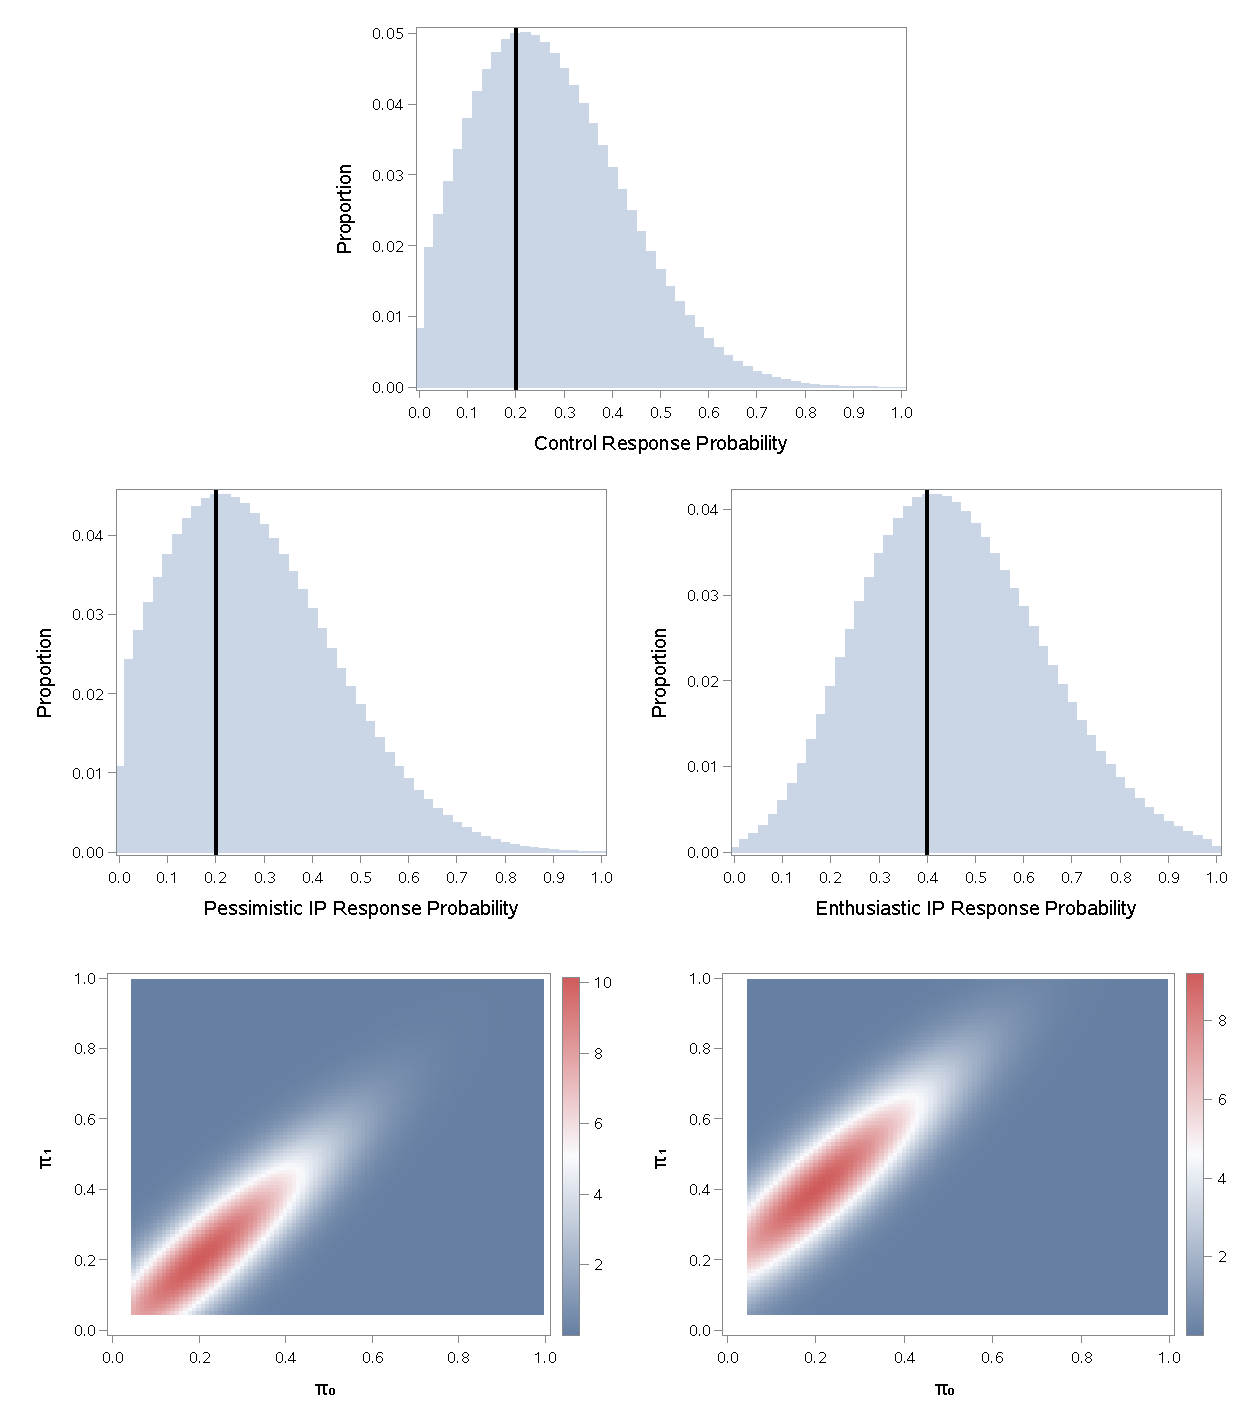
\includegraphics[scale=0.70]{./FIGURES/BINARY-PRIORS.pdf}
%      \caption{Prior for Control Group Response Probability \label{fig:pmp}}
%    \end{figure}
			
	

%\bigskip
\newpage
\begin{center}
{\large\bf SUPPLEMENTARY MATERIAL}
\end{center}


\section{BibTeX}

 \bibliographystyle{agsm}
 \bibliography{./References}		

\end{document}
